\documentclass[../DoAn.tex]{subfiles}
\begin{document}

\section{Khảo sát hiện trạng}
\label{section:2.1}
Trên thị trường ứng dụng Android và iOS đã xuất hiện một số ứng dụng có thể cho phép kết nối với các thiết bị Arduino, thiết lập một số tính năng và điều khiển thiết bị. Dưới đây là hai ứng dụng em đã tìm hiểu. Đầu tiên là ứng dụng Blynk \cite{Blynk}, một ứng dụng tương đối nổi tiếng của nước ngoài, theo thống kê của ứng dụng này, đã có 800,000 thiết bị đã kết nối, 300 triệu tin nhắn từ phần cứng và hơn 1,5 triệu lượt tải ứng dụng Blynk. Ứng dụng thứ hai là ESP32 Camera Wifi Robot Car mới ra đời với rất nhiều lượt tải xuống, có thể kể tới đó là: 4 sao đánh giá, trên 5,000 lượt tải.

Với ứng dụng Blynk, người dùng có thể xây dựng giao diện bằng việc kéo thả các thành phần, thêm chức năng cho các thành phần đó. Bên cạnh đó, ứng dụng giúp người dùng quản lý nhiều loại thiết bị như ESP32, Arduino, Respberry Pi, ... kết nối chúng tới điện toán đám mây, kết hợp với giao diện trực quan để điều khiển các phần cứng đó. Tuy nhiên với việc sử dụng Blynk, người dùng sẽ phải sử dụng server của họ, rất bất tiện trong việc người lập trình muốn chỉnh sửa cấu trúc, logic sao cho phù hợp với hệ thống điều khiển của mình.

\begin{figure}[H]
    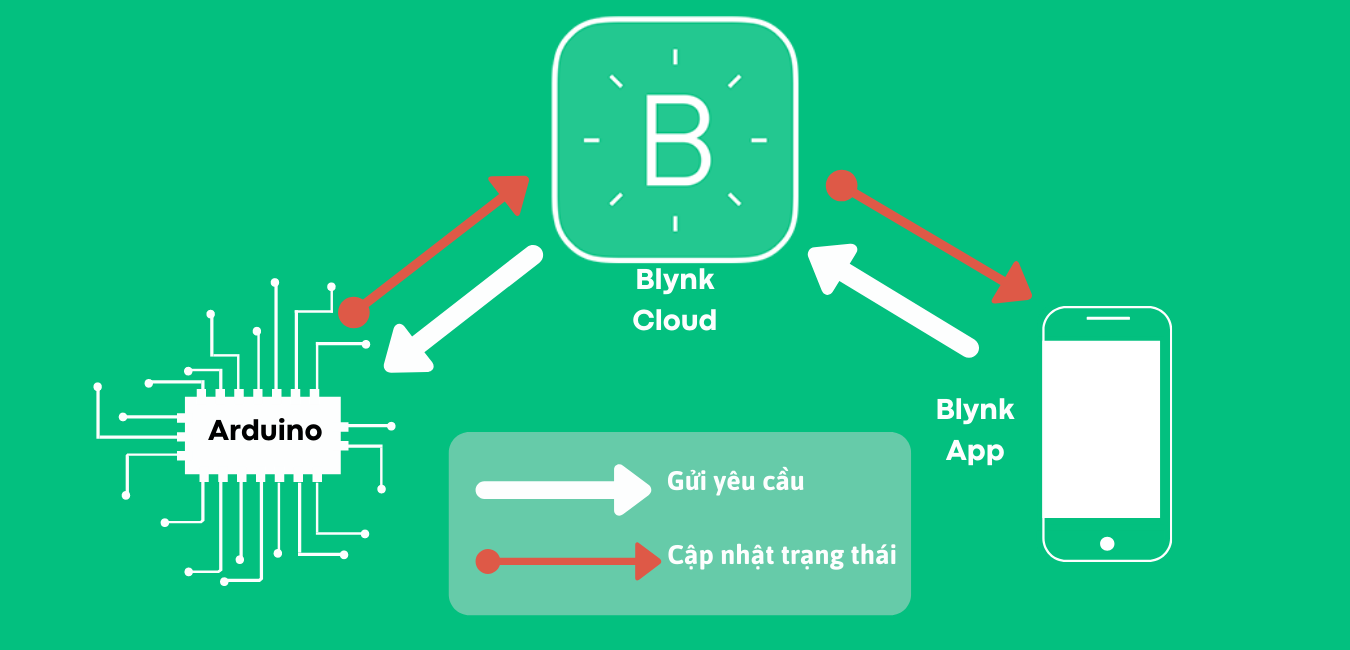
\includegraphics[scale = 0.4]{Hinhve/blynk.png}
    \centering
    \caption{Sơ đồ mô tả kết nối các thiết bị sử dụng Blynk}
\end{figure}

Còn về ứng dụng ESP32 Camera Wifi Robot Car, ứng dụng được xây dựng giúp người dùng dễ dàng kết nối tới một chiếc xe robot có camera và có thể quan sát qua ứng dụng. Ứng dụng cho phép người dùng điều khiển ESP32-Cam, người dùng có thể đẩy mã nguồn tới ESP32-Cam bằng USB OTG hoặc qua Wifi. Tuy nhiên, phần giao diện điều khiển của ứng dụng còn chưa trực quan và đẹp mắt, đồng thời, mã nguồn từ ứng dụng không thể chỉnh sửa theo ý người dùng, chỉ được chỉnh sửa tên và mật khẩu của Wifi. Ứng dụng phù hợp cho những người mới tiếp xúc với Arduino và đang tìm hiểu về điều khiển thiết bị qua Wifi.

\begin{figure}[!h]
    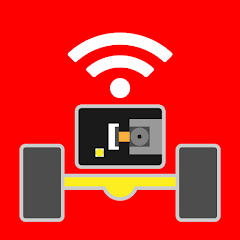
\includegraphics[scale = 1]{Hinhve/wif_robot_car.png}
    \centering
    \caption{Ứng dụng ESP32 Camera Wifi Robot Car}
\end{figure}

Từ những so sánh trên, em sẽ phát triển hệ thống điều khiển xe Arduino bằng ứng dụng đa nền tảng Flutter với các chức năng cơ bản của ứng dụng như điều khiển xe, thiết lập tốc độ xe và có thể điều khiển bằng giọng nói với giao diện trực quan, dễ sử dụng đặc biệt cho người mới bắt đầu. Ứng dụng có thể hoạt động được trên nhiều nền tảng như Android, iOS và Web. Xe Arduino nhận tín hiệu di chuyển từ phía ứng dụng và thực hiện di chuyển, cảm biến khoảng cách và cảnh báo người dùng. Đặc biệt ứng dụng có thể điều khiển xe với độ trễ thấp, mang lại trải nghiệm tốt về sản phẩm.

\section{Tổng quan chức năng}
\label{section:2.2}

\subsection{Biểu đồ use case tổng quát}
\label{subsection:2.2.1}
\begin{figure}[H]
    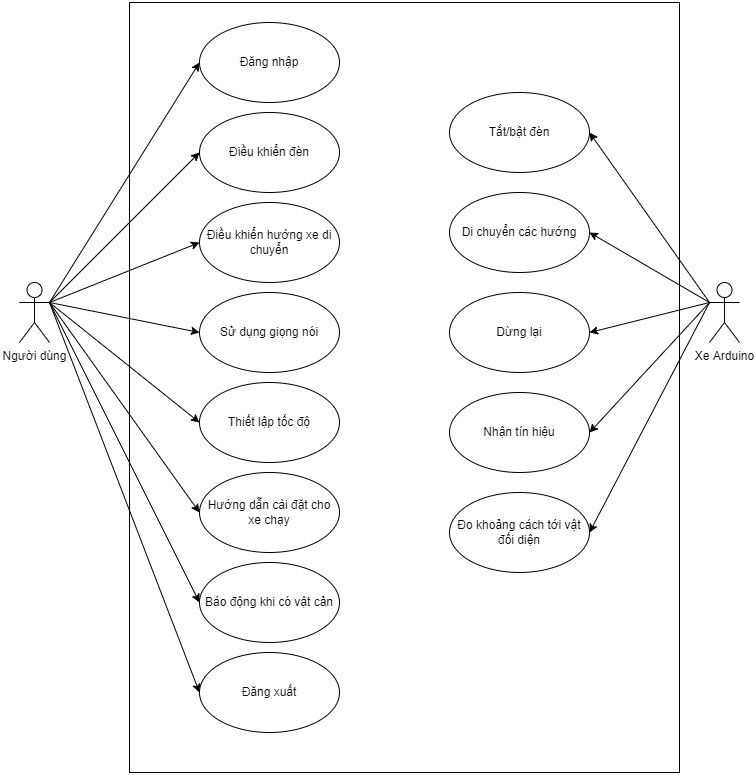
\includegraphics[scale = 0.6]{Hinhve/usecase_tong_quan.png}
    \centering
    \caption{Biểu đồ use case tổng quát}
    \label{fig:2.2.1}
\end{figure}

Hình \ref{fig:2.2.1} mô tả use case tổng quan của hệ thống điều khiển xe Arduino. Bao gồm 2 tác nhân với 2 vai trò khác nhau: Người dùng và xe Arduino. Với vai trò là người dùng, người dùng có các chức năng sau:
\begin{itemize}
    \item Đăng nhập: Người dùng lựa chọn server cần kết nối.
    \item Điều khiển đèn: Người dùng tắt/bật đèn Led.
    \item Điều khiển hướng xe di chuyển.
    \item Sử dụng giọng nói điều khiển cho xe.
    \item Thiết lập tốc độ chạy cho xe.
    \item Hướng dẫn cài đặt cho xe chạy với người mới sử dụng.
    \item Báo động khi xe Arduino gặp vật cản.
    \item Đăng xuất: Thoát khỏi kết nối.
\end{itemize}

\subsection{Biểu đồ use case phân rã}
\label{subsection:2.2.2}

\subsubsection{Biểu đồ use case Điều khiển xe các hướng}
\label{subsection:2.2.2.1}

Hình \ref{fig:2.2.2.1} mô tả use case phân rã của use case điều khiển xe các hướng. Người dùng sẽ thực hiện chức năng sử dụng bộ điều khiển di chuyển các hướng và có thể thiết lập tốc độ cho xe Arduino. Xe Arduino sẽ nhận tín hiệu và thực hiện chức năng theo yêu cầu người dùng là di chuyển theo các hướng yêu cầu, dừng lại.

\begin{figure}[H]
    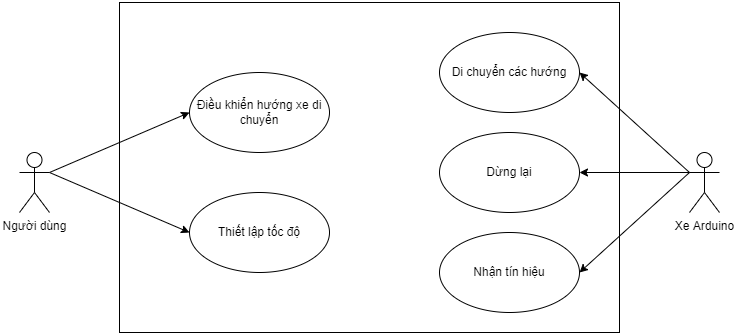
\includegraphics[scale = 0.6]{Hinhve/usecase_phan_ra_dieu_khien_xe.png}
    \centering
    \caption{Biểu đồ use case phân rã Điều khiển xe các hướng}
    \label{fig:2.2.2.1}
\end{figure}

\subsubsection{Biểu đồ use case Điều khiển đèn LED}
\label{subsection:2.2.2.2}

Hình \ref{fig:2.2.2.2} mô tả use case phân rã của use case điều khiển đèn LED. 

Với vai trò người dùng, họ sử dụng nút ấn để tắt/bật đèn, có thể đổi màu cho đèn, nháy đèn. Về phía xe Arduino, nó lắng nghe tín hiệu và thực hiện tắt/bật đèn theo, đổi màu đèn theo yêu cầu và thêm chức năng nháy đèn.

\begin{figure}[H]
    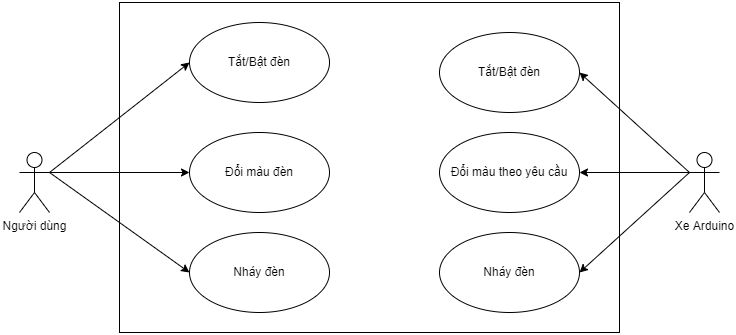
\includegraphics[scale = 0.6]{Hinhve/usecase_phan_ra_dieu_khien_den.png}
    \centering
    \caption{Biểu đồ use case phân rã Điều khiển đèn LED}
    \label{fig:2.2.2.2}
\end{figure}

\subsubsection{Biểu đồ use case Báo hiệu xe gặp vật cản}
\label{subsection:2.2.2.3}

Hình \ref{fig:2.2.2.3} mô tả use case phân rã của use case báo hiệu xe gặp vật cản.

Khi người dùng điều khiển xe di chuyển, xe Arduino có thể gặp vật cản, họ sẽ nhận được tín hiệu báo động. Xe Arduino khi gặp vật cản trước mặt sẽ dừng lại, nháy đèn báo động cho người dùng được biết.

\begin{figure}[H]
    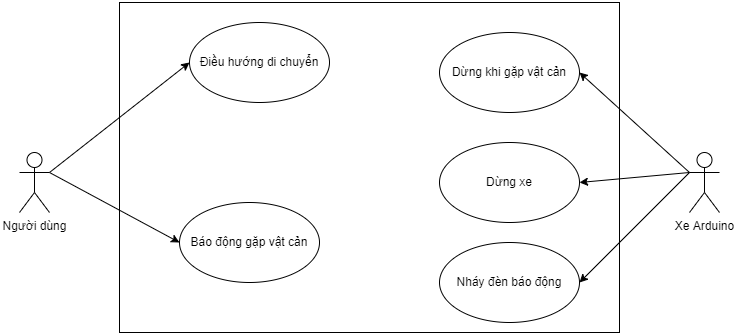
\includegraphics[scale = 0.6]{Hinhve/usecase_phan_ra_cam_bien_khoang_cach.png}
    \centering
    \caption{Biểu đồ use case phân rã Báo hiệu xe gặp vật cản}
    \label{fig:2.2.2.3}
\end{figure}

\subsection{Quy trình nghiệp vụ}
\label{subsection:2.2.3}
\subsubsection{Quy trình điều khiển hướng xe di chuyển}
\label{subsection:2.2.3.1}
\begin{figure}[H]
    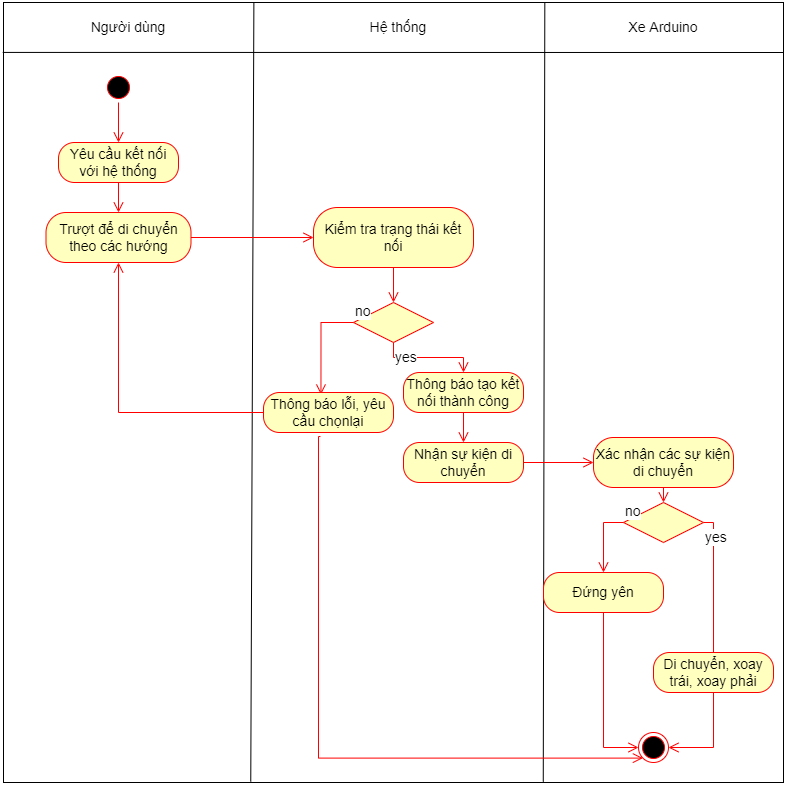
\includegraphics[scale = 0.6]{Hinhve/activity_dieu_khien_xe.png}
    \centering
    \caption{Biểu đồ hoạt động quy trình điều khiển hướng xe di chuyển}
    \label{fig:2.2.3.1}
\end{figure}
Hình \ref{fig:2.2.3.1} là quy trình điều khiển hướng xe Arduino di chuyển, người dùng phải kết nối được hệ thống trước khi thực hiện trượt bộ điều khiển nếu không chiếc xe không thể di chuyển.

Để điều khiển được xe, người dùng thực hiện các bước: (i) Bước 1: Người dùng lựa chọn hệ thống cần kết nối và xe Arduino đã được kết nối trước đó. (ii) Bước 2: Người dùng trượt các hướng trên màn hình để di chuyển. Khi đó, tín hiệu đã được truyền tới xe Arduino. (iii) Bước 3: Xe Arduino di chuyển theo hướng di chuyển của người dùng điều khiển.

\subsubsection{Quy trình điều khiển đèn}
\label{subsection:2.2.3.2}
\begin{figure}[H]
    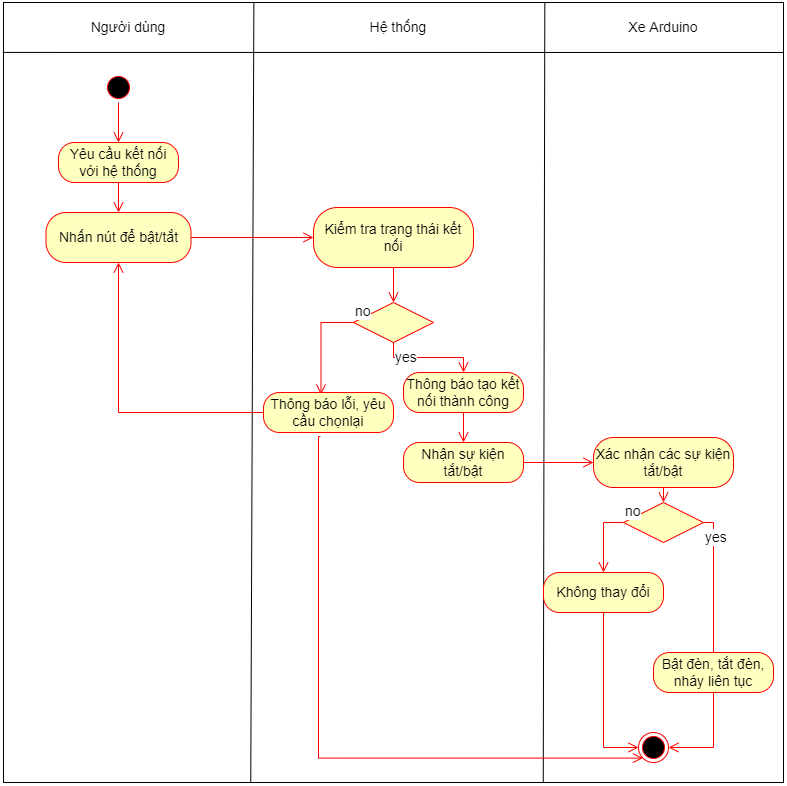
\includegraphics[scale = 0.6]{Hinhve/activity_dieu_khien_den.png}
    \centering
    \caption{Biểu đồ hoạt động quy trình điều khiển đèn}
    \label{fig:2.2.3.2}
\end{figure}

Hình \ref{fig:2.2.3.2} là quy trình điều khiển đèn LED trên xe, người dùng phải kết nối được hệ thống trước khi thực hiện ấn nút tắt/bật nếu không đèn LED sẽ không phản hồi.

Để điều khiển được đèn LED, người dùng thực hiện các bước: (i) Bước 1: Người dùng lựa chọn hệ thống cần kết nối và xe Arduino đã được kết nối trước đó. (ii) Bước 2: Người dùng ấn nút trên màn hình để tắt/bật. Khi đó, tín hiệu đã được truyền tới xe Arduino. (iii) Bước 3: Đèn LED tắt/bật theo lựa chọn của người dùng điều khiển.

\subsubsection{Quy trình Báo động khi xe gặp vật cản}
\label{subsection:2.2.3.3}
\begin{figure}[H]
    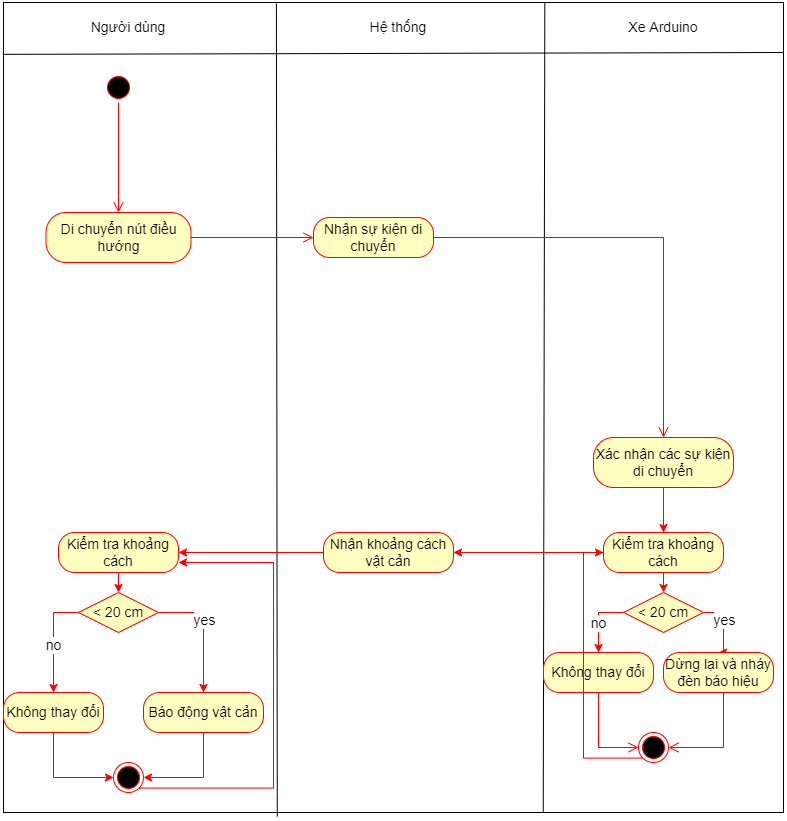
\includegraphics[scale = 0.6]{Hinhve/activity_bao_dong_vat_can.png}
    \centering
    \caption{Biểu đồ hoạt động quy trình Báo động khi xe gặp vật cản}
    \label{fig:2.2.3.3}
\end{figure}

Hình \ref{fig:2.2.3.3} là quy trình báo động khi xe gặp vật cản. Khi người dùng thực hiện điều hướng con trỏ, xe sẽ có các nhiệm vụ sau: (i) Xe Arduino di chuyển theo yêu cầu người dùng, (ii) Xe sẽ luôn kiểm tra khoảng cách giữa xe tới vật phía trước và gửi tín hiệu liên tục về người dùng, (iii) Xe phát hiện nếu khoảng cách nhỏ hơn 20cm sẽ dừng lại và nháy đèn báo hiệu. Lúc này người dùng sẽ nhận được báo động gặp vật cản.

\section{Đặc tả chức năng}
\label{section:2.3}
Em sẽ đặc tả chi tiết một số use case chính là: Điều khiển hướng xe, Điều khiển đèn, Điều khiển bằng giọng nói.
\subsection{Đặc tả use case điều khiển hướng xe di chuyển}
\hfill
% Please add the following required packages to your document preamble:
% \usepackage{graphicx}
% \usepackage[table,xcdraw]{xcolor}
% If you use beamer only pass "xcolor=table" option, i.e. \documentclass[xcolor=table]{beamer}
\begin{table}[H]
\resizebox{\columnwidth}{!}{%
\begin{tabular}{| p{1.5cm} | p{1cm} | p{1.5cm} | p{10cm} |}
\hline
\multicolumn{1}{|l|}{\cellcolor[HTML]{9AFF99}\textbf{Mã Use case}} &
  \multicolumn{1}{l|}{\textbf{UC001}} &
  \multicolumn{1}{l|}{\textbf{Tên Use case}} &
  \textbf{Điều khiển hướng xe} \\ \hline
\multicolumn{1}{|l|}{\cellcolor[HTML]{9AFF99}\textbf{Tác nhân}} &
  \multicolumn{3}{l|}{Người dùng, Xe Arduino} \\ \hline
\multicolumn{1}{|l|}{\cellcolor[HTML]{9AFF99}\textbf{Tiền điều kiện}} &
  \multicolumn{3}{l|}{Kết nối với hệ thống} \\ \hline
\multicolumn{4}{|l|}{\textbf{Điều khiển hướng}} \\ \hline
\multicolumn{1}{|l|}{} &
  \multicolumn{1}{l|}{\cellcolor[HTML]{FFCE93}STT} &
  \multicolumn{1}{l|}{\cellcolor[HTML]{FFCE93}Thực hiện bởi} &
  \cellcolor[HTML]{FFCE93}Hành động \\ \hline
\multicolumn{1}{|l|}{\cellcolor[HTML]{9AFF99}} &
  \multicolumn{1}{l|}{1} &
  \multicolumn{1}{l|}{Người dùng} &
  Trượt con trỏ theo các hướng \\ \cline{2-4} 
\multicolumn{1}{|l|}{\cellcolor[HTML]{9AFF99}} &
  \multicolumn{1}{l|}{2} &
  \multicolumn{1}{l|}{Hệ thống} &
  Hiển thị con trỏ theo hướng đó \\ \cline{2-4} 
\multicolumn{1}{|l|}{\cellcolor[HTML]{9AFF99}} &
  \multicolumn{1}{l|}{3} &
  \multicolumn{1}{l|}{Hệ thống} &
  Nhận tín hiệu di chuyển \\ \cline{2-4} 
\multicolumn{1}{|l|}{\cellcolor[HTML]{9AFF99}} &
  \multicolumn{1}{l|}{4} &
  \multicolumn{1}{l|}{Xe Arduino} &
  Phát hiện tín hiệu từ hệ thống, di chuyển theo hướng đã truyền \\ \cline{2-4} 
\multicolumn{1}{|l|}{\cellcolor[HTML]{9AFF99}\textbf{Luồng sự kiện thay thế}} &
  \multicolumn{1}{l|}{} &
  \multicolumn{1}{l|}{} &
   \\ \hline
\end{tabular}%
}
\caption{Đặc tả use case Điều khiển hướng xe di chuyển}
\end{table}

\subsection{Đặc tả use case điều khiển đèn LED}
\hfill

\begin{table}[H]
\resizebox{\columnwidth}{!}{%
\begin{tabular}{| p{1.5cm} | p{1cm} | p{1.5cm} | p{10cm} |}
\hline
\multicolumn{1}{|l|}{\cellcolor[HTML]{9AFF99}\textbf{Mã Use case}} &
  \multicolumn{1}{l|}{\textbf{UC002}} &
  \multicolumn{1}{l|}{\textbf{Tên Use case}} &
  \textbf{Điều khiển đèn LED} \\ \hline
\multicolumn{1}{|l|}{\cellcolor[HTML]{9AFF99}\textbf{Tác nhân}} &
  \multicolumn{3}{l|}{Người dùng, Xe Arduino} \\ \hline
\multicolumn{1}{|l|}{\cellcolor[HTML]{9AFF99}\textbf{Tiền điều kiện}} &
  \multicolumn{3}{l|}{Kết nối với hệ thống} \\ \hline
\multicolumn{4}{|l|}{\textbf{Điều khiển đèn LED}} \\ \hline
\multicolumn{1}{|l|}{} &
  \multicolumn{1}{l|}{\cellcolor[HTML]{FFCE93}STT} &
  \multicolumn{1}{l|}{\cellcolor[HTML]{FFCE93}Thực hiện bởi} &
  \cellcolor[HTML]{FFCE93}Hành động \\ \hline
\multicolumn{1}{|l|}{\cellcolor[HTML]{9AFF99}} &
  \multicolumn{1}{l|}{1} &
  \multicolumn{1}{l|}{Người dùng} &
  Nhấn nút tắt/bật \\ \cline{2-4} 
\multicolumn{1}{|l|}{\cellcolor[HTML]{9AFF99}} &
  \multicolumn{1}{l|}{2} &
  \multicolumn{1}{l|}{Hệ thống} &
  Hiển thị nút đậm là đang bật, xám là đang tắt \\ \cline{2-4} 
\multicolumn{1}{|l|}{\cellcolor[HTML]{9AFF99}} &
  \multicolumn{1}{l|}{3} &
  \multicolumn{1}{l|}{Hệ thống} &
  Nhận tín hiệu tắt/bật \\ \cline{2-4} 
\multicolumn{1}{|l|}{\cellcolor[HTML]{9AFF99}} &
  \multicolumn{1}{l|}{4} &
  \multicolumn{1}{l|}{Xe Arduino} &
  Phát hiện tín hiệu từ hệ thống, đèn LED tắt/bật theo tín hiệu đã truyền \\ \cline{2-4} 
\multicolumn{1}{|l|}{\cellcolor[HTML]{9AFF99}\textbf{Luồng sự kiện thay thế}} &
  \multicolumn{1}{l|}{} &
  \multicolumn{1}{l|}{} &
   \\ \hline
\end{tabular}%
}
\caption{Đặc tả use case Điều khiển đèn LED}
\end{table}

\subsection{Đặc tả use case điều khiển bằng giọng nói}
\hfill

\begin{table}[H]
\resizebox{\columnwidth}{!}{%
\begin{tabular}{| p{1.5cm} | p{1cm} | p{1.5cm} | p{10cm} |}
\hline
\multicolumn{1}{|l|}{\cellcolor[HTML]{9AFF99}\textbf{Mã Use case}} &
  \multicolumn{1}{l|}{\textbf{UC001}} &
  \multicolumn{1}{l|}{\textbf{Tên Use case}} &
  \textbf{Điều khiển bằng giọng nói} \\ \hline
\multicolumn{1}{|l|}{\cellcolor[HTML]{9AFF99}\textbf{Tác nhân}} &
  \multicolumn{3}{l|}{Người dùng, Xe Arduino} \\ \hline
\multicolumn{1}{|l|}{\cellcolor[HTML]{9AFF99}\textbf{Tiền điều kiện}} &
  \multicolumn{3}{l|}{Kết nối với hệ thống} \\ \hline
\multicolumn{4}{|l|}{\textbf{Điều khiển bằng giọng nói}} \\ \hline
\multicolumn{1}{|l|}{} &
  \multicolumn{1}{l|}{\cellcolor[HTML]{FFCE93}STT} &
  \multicolumn{1}{l|}{\cellcolor[HTML]{FFCE93}Thực hiện bởi} &
  \cellcolor[HTML]{FFCE93}Hành động \\ \hline
\multicolumn{1}{|l|}{\cellcolor[HTML]{9AFF99}} &
  \multicolumn{1}{l|}{1} &
  \multicolumn{1}{l|}{Người dùng} &
  Ra lệnh bằng giọng nói \\ \cline{2-4} 
\multicolumn{1}{|l|}{\cellcolor[HTML]{9AFF99}} &
  \multicolumn{1}{l|}{2} &
  \multicolumn{1}{l|}{Hệ thống} &
  Thu âm giọng nói, phân tích từ xem có từ để điều khiển xe hay không \\ \cline{2-4} 
\multicolumn{1}{|l|}{\cellcolor[HTML]{9AFF99}} &
  \multicolumn{1}{l|}{3} &
  \multicolumn{1}{l|}{Hệ thống} &
  Nhận tín hiệu di chuyển hoặc tắt/bật đèn \\ \cline{2-4} 
\multicolumn{1}{|l|}{\cellcolor[HTML]{9AFF99}} &
  \multicolumn{1}{l|}{4} &
  \multicolumn{1}{l|}{Xe Arduino} &
  Phát hiện tín hiệu từ hệ thống, di chuyển theo hướng đã truyền hoặc tắt/bật đèn LED \\ \cline{2-4} 
\multicolumn{1}{|l|}{\cellcolor[HTML]{9AFF99}\textbf{Luồng sự kiện thay thế}} &
  \multicolumn{1}{l|}{} &
  \multicolumn{1}{l|}{} &
   \\ \hline
\end{tabular}%
}
\caption{Đặc tả use case Điều khiển bằng giọng nói}
\end{table}

\subsection{Đặc tả use case Báo động khi xe gặp vật cản}
\hfill

\begin{table}[H]
\resizebox{\columnwidth}{!}{%
\begin{tabular}{| p{1.5cm} | p{1cm} | p{1.5cm} | p{10cm} |}
\hline
\multicolumn{1}{|l|}{\cellcolor[HTML]{9AFF99}\textbf{Mã Use case}} &
  \multicolumn{1}{l|}{\textbf{UC002}} &
  \multicolumn{1}{l|}{\textbf{Tên Use case}} &
  \textbf{Báo động khi xe gặp vật cản} \\ \hline
\multicolumn{1}{|l|}{\cellcolor[HTML]{9AFF99}\textbf{Tác nhân}} &
  \multicolumn{3}{l|}{Người dùng, Xe Arduino} \\ \hline
\multicolumn{1}{|l|}{\cellcolor[HTML]{9AFF99}\textbf{Tiền điều kiện}} &
  \multicolumn{3}{l|}{Kết nối với hệ thống} \\ \hline
\multicolumn{4}{|l|}{Báo động khi xe gặp vật cản} \\ \hline
\multicolumn{1}{|l|}{} &
  \multicolumn{1}{l|}{\cellcolor[HTML]{FFCE93}STT} &
  \multicolumn{1}{l|}{\cellcolor[HTML]{FFCE93}Thực hiện bởi} &
  \cellcolor[HTML]{FFCE93}Hành động \\ \hline
\multicolumn{1}{|l|}{\cellcolor[HTML]{9AFF99}} &
  \multicolumn{1}{l|}{1} &
  \multicolumn{1}{l|}{Người dùng} &
  Di chuyển xe đi \\ \cline{2-4} 
\multicolumn{1}{|l|}{\cellcolor[HTML]{9AFF99}} &
  \multicolumn{1}{l|}{2} &
  \multicolumn{1}{l|}{Hệ thống} &
  Hiển thị con trỏ theo hướng đó \\ \cline{2-4} 
\multicolumn{1}{|l|}{\cellcolor[HTML]{9AFF99}} &
  \multicolumn{1}{l|}{3} &
  \multicolumn{1}{l|}{Xe Arduino} &
  Di chuyển theo các hướng \\ \cline{2-4} 
\multicolumn{1}{|l|}{\cellcolor[HTML]{9AFF99}} &
  \multicolumn{1}{l|}{4} &
  \multicolumn{1}{l|}{Xe Arduino} &
  Đo khoảng cách liên tục từ xe tới vật cản \\ \cline{2-4} 
\multicolumn{1}{|l|}{\cellcolor[HTML]{9AFF99}} &
  \multicolumn{1}{l|}{4} &
  \multicolumn{1}{l|}{Hệ thống} &
  Hiển thị khoảng cách mà Arduino báo về \\ \cline{2-4} 
\multicolumn{1}{|l|}{\cellcolor[HTML]{9AFF99}} &
  \multicolumn{1}{l|}{4} &
  \multicolumn{1}{l|}{Xe Arduino} &
  Dừng lại và báo đèn đỏ khi gặp vật cản \\ \cline{2-4} 
\multicolumn{1}{|l|}{\cellcolor[HTML]{9AFF99}} &
  \multicolumn{1}{l|}{4} &
  \multicolumn{1}{l|}{Hệ thống} &
  Báo động cho người dùng biết \\ \cline{2-4} 
\multicolumn{1}{|l|}{\cellcolor[HTML]{9AFF99}\textbf{Luồng sự kiện thay thế}} &
  \multicolumn{1}{l|}{} &
  \multicolumn{1}{l|}{} &
   \\ \hline
\end{tabular}%
}
\caption{Đặc tả use case Báo động khi xe gặp vật cản}
\end{table}

\section{Yêu cầu phi chức năng}
\label{section:2.4}

\subsection{Tính dễ dùng, thân thiện người dùng}
\label{section:2.4.1}
Do ứng dụng được xây dựng dựa vào Flutter nên giao diện được thiết kế đẹp mắt, mượt mà và trực quan, thuận tiện trong việc sử dụng ứng dụng của người dùng. Bố cục trình bày nhất quán giữa các chức năng, hiển thị thông báo đầy đủ. Việc hiển thị dữ liệu cần được đảm bảo thời gian nhanh, tránh người dùng phải đợi. Đặc biệt, cần hỗ trợ hiển thị trên các trình duyệt máy tính cũng như thiết bị di động bao gồm Android và iOS.
\subsection{Tính bảo mật}
\label{section:2.4.2}
Dữ liệu trong hệ thống cần được bảo vệ và xác thực người dùng trước khi được sử dụng.
\subsection{Tính dễ bảo trì, nâng cấp}
\label{section:2.4.4}
Hệ thống cần được thiết kế sao cho hạn chế lỗi nhất có thể, nếu có lỗi phải thông báo rõ ràng để người dùng được biết cũng như người lập trình dễ sửa lỗi, bên cạnh đó chi phí bảo trì tối thiểu nhất có thể. Đồng thời ứng dụng dễ dàng nâng cấp về sau.


%%%%%%%%%%%%%%%%%%%%%%%%%%%%%%%%%%%

\end{document}